% vim:encoding=utf8 ft=tex sts=2 sw=2 et:

\documentclass{classrep}
\usepackage[utf8]{inputenc}
\usepackage{color}
\usepackage{mathtools}

\usepackage{subfig}
\usepackage{float}

\usepackage[labelfont=it]{caption}

\studycycle{Informatyka, studia niestacjonarne, mgr II st.}
\coursesemester{I}

\coursename{Przetwarzanie obrazu i dźwięku}
\courseyear{2015/2016}

\courseteacher{mgr inż. Piotr Ożdżyński}
\coursegroup{Sobota, 14:15}

\author{
  \studentinfo{Jakub Antosik}{206788} \and
  \studentinfo{Andrzej Lisowski}{206807} 
}

\title{Zadanie 1: Szkielet aplikacji do przetwarzania i analizy obrazów, operacje podstawowe, usuwanie szumu,
modyfikacje histogramu, filtracja liniowa i nieliniowa, splot.}

\begin{document}
\maketitle

\section{Cel}
Celem zadania było zapoznanie się z metodami analizy i przetwarzania obrazów. W części implementacyjnej należało stworzyć program w wybranym przez siebie języku programowania, który będzie w stanie przeprowadzić różne operacje na obrazie. Pełen spis funkcjonalności zostanie przedstawiony w sekcji \textit{Wprowadzenie}.

\section{Wprowadzenie}
Obraz w pamięci komputera jest reprezentowany przez macierz pikseli. Sam piksel jest zaś najmniejszym elementem obrazu, mogącym przyjmować różne wartości liczb naturalnych:
\begin{itemize}
\item 0 - 7 dla obrazów 1-bitowych
\item 0 - 255 dla obrazów 8-bitowych (odcienie szarości)
\item 0 - 16777215 dla obrazów 24-bitowych (po 8 bitów na każdy kolor RGB)
\end{itemize}
Poniżej przedstawione zostały teoretyczne podstawy trasformacji, którym poddane zostały testowe dane.

\subsection{Podstawowe operacje przetwarzania obrazu}
Sekcja ta opisuje podstawowe operacje przetwarzania obrazów, często wykorzystywane w codziennym życiu.

\subsubsection{Zmiana jasności}
Zmiana jasności obrazu polega na dodaniu do wartości każdego piksela pewnej stałej liczby k. Jeżeli stała jest dodatnia, mówimy o zwiększaniu jasności, jeżeli jest ujemna - jasność jest zmniejszana. W momencie, w którym wynik przekroczy wartości brzegowe piksela, przypisuje się mu p$_{\text{min}}$ lub p$_{\text{max}}$. Wzór jest następujący:
\[ p(i) =
  \begin{cases}
    p_{min} & \quad \text{jeżeli } i + k < 0\\
    i + k  & \quad \text{jeżeli } p_{min} \leq i+k \leq p_{max}\\
    p_{max}  & \quad \text{jeżeli } i + k > 0\\
  \end{cases}
\]
gdzie:\\
\textit{p(i)} - wartość piksela po zmianie jasności,\\
\textit{i} - wartość piksela przed zmianą jasności,\\
\textit{p$_{\text{min}}$} - minimalna wartość piksela, p$_{\text{min}}$ = 0,\\
\textit{p$_{\text{max}}$} - maksymalna wartość piksela,\\
\textit{k} - zmiana jasności.\\

\subsubsection{Zmiana kontrastu}
Zmiana kontrastu obrazu polega na zwiększeniu jasności jasnych pikseli przy jednoczesnym zmniejszeniu jasności ciemnych pikseli. Ciemne piksele należą do przedziału $\langle$0,$ \frac{p_{max}}{2}$), zaś jasne do przedziału $\langle$$ \frac{p_{max}}{2}$,$p_{max}$$\rangle$.\\
\\
Ogólny wzór wygląda następująco:
\[ p(i) =
  \begin{cases}
    i \div k  & \quad \text{jeżeli } 0 \leq i < \frac{p_{max}}{2}\\
    i \ast k  & \quad \text{jeżeli } \frac{p_{max}}{2} \leq i \leq p_{max}\\
    p_{max}  & \quad \text{jeżeli } i \ast k > p_{max}\\
  \end{cases}
\]
gdzie:\\
\textit{p(i)} - wartość piksela po zmianie kontrastu,\\
\textit{i} - wartość piksela przed zmianą kontrastu,\\
\textit{p$_{\text{max}}$} - maksymalna wartość piksela,\\
\textit{k} - współczynnik zmiany kontrastu.\\

\subsubsection{Wyznaczenie negatywu}
Negatyw jest przedstawieniem pikseli obrazu jako różnicy wartości maksymalnej i obecnej:\\
\\
\[p(i) = p_{max} - i\]
gdzie:\\
\textit{p(i)} - wartość piksela po wyznaczeniu negatywu,\\
\textit{i} - wartość piksela przed zmianą kontrastu,\\
\textit{p$_{\text{max}}$} - maksymalna wartość piksela.\\

\subsection{Podstawowe filtry}
Poniższa sekcja opisuje 2 podstawowe filtry, które podległy analizie - filtr ze średnią arytmetyczną oraz filtr medianowy.

\subsubsection{Filtr ze średnią arytmetyczną}
Filtr ze średnią arytmetyczną jest wykorzystywany w operacjach odszumiania obrazu. Algorytm polega na przypisaniu do nowej wartości pikseli średniej arytmetycznej badanego elementu oraz jego sąsiedztwa s. Sąsiedztwo może przyjmować wartości potęg kolejnych liczb nieparzystych większych od 1:\\
\[ s \in \{9,25,49,...\} \]
\[ p(i) = \frac{\displaystyle\sum_{x=-n}^{n}\displaystyle\sum_{y=-n}^{n} i_{x,y}}{s} \]
gdzie:\\
\textit{p(i)} - wartość piksela po nałożeniu filtru,\\
\textit{i} - wartość piksela przed nałożeniem filtru,\\
\textit{s} - maska filtru,\\
\textit{n} - rozpiętość maski filtru, obliczana ze wzoru:\\
\[ n = \frac{\sqrt{s}-1}{2} \]
\textit{x} - współrzędna x piksela na obrazie,\\
\textit{y} - współrzędna y piksela na obrazie.\\
\\
Należy pamiętać, że piksele poddawane filtracji nie mogą być elementami brzegowymi obrazu, więc:
\[ i_x + n \leq x_{max} \wedge i_x - n \geq x_{min} \wedge i_y + n \leq y_{max} \wedge i_y - n \geq y_{min} \]
gdzie:\\
\textit{i} - wartość piksela przed zmianą kontrastu,\\
\textit{x} - współrzędna x piksela na obrazie,\\
\textit{y} - współrzędna y piksela na obrazie,\\
\textit{x$_{\text{max}}$} - maksymalna wartość współrzędnej x na obrazie,\\
\textit{x$_{\text{min}}$} - minimalna wartość współrzędnej x na obrazie, x$_{\text{min}}$ = 0,\\
\textit{y$_{\text{max}}$} - maksymalna wartość współrzędnej y na obrazie,\\
\textit{y$_{\text{min}}$} - minimalna wartość współrzędnej y na obrazie, y$_{\text{min}}$ = 0.\\

\subsubsection{Filtr medianowy}
Filtr medianowy jest bardzo podobny do filtru ze średnią arytmetyczną. W tym przypadku jednak, nowa wartość piksela jest medianą badanego elementu oraz jego sąsiedztwa s. Sąsiedztwo może przyjmować wartości potęg kolejnych liczb nieparzystych większych od 1:\\
\[ s \in \{9,25,49,...\} \]
\[ p(i) = M_{s} \]
gdzie:\\
\textit{p(i)} - wartość piksela po nałożeniu filtru,\\
\textit{M} - mediana,\\
\textit{s} - maska filtru.\\
\\
Należy pamiętać, że piksele poddawane filtracji nie mogą być elementami brzegowymi obrazu, więc:
\[ i_x + n \leq x_{max} \wedge i_x - n \geq x_{min} \wedge i_y + n \leq y_{max} \wedge i_y - n \geq y_{min} \]
gdzie:\\
\textit{i} - wartość piksela przed zmianą kontrastu,\\
\textit{n} - rozpiętość maski filtru, obliczana ze wzoru:\\
\[ n = \frac{\sqrt{s}-1}{2} \]
\textit{x} - współrzędna x piksela na obrazie,\\
\textit{y} - współrzędna y piksela na obrazie,\\
\textit{x$_{\text{max}}$} - maksymalna wartość współrzędnej x na obrazie,\\
\textit{x$_{\text{min}}$} - minimalna wartość współrzędnej x na obrazie, x$_{\text{min}}$ = 0,\\
\textit{y$_{\text{max}}$} - maksymalna wartość współrzędnej y na obrazie,\\
\textit{y$_{\text{min}}$} - minimalna wartość współrzędnej y na obrazie, y$_{\text{min}}$ = 0.\\

\subsection{Modyfikacje obrazu w oparciu o histogram}
Histogram umożliwia przedstawienie rozkładu pikseli o określonych wartościach na wykresie. Poniższa sekcja prezentuje modyfikacje obrazu na podstawie jego histogramu.

\subsubsection{Jednostajna wyjściowa gęstość prawdopodobieństwa}
Obliczana jest ze wzoru:
\[ g(f) = g_{min} + (g_{max} - g_{min}) \frac{1}{N} \displaystyle\sum_{m=0}^{f} H(m) \]
gdzie:\\
\textit{f} - wartość rozważanego kanału przed modyfikacją,\\
\textit{g} - wartość rozważanego kanału po modyfikacji,\\
\textit{g$_{\text{min}}$} - pożądana minimalna wartość przetwarzanego kanału,\\
\textit{g$_{\text{max}}$} - pożądana maksymalna wartość przetwarzanego kanału,\\
\textit{N} - suma pikseli na obrazie,\\
\textit{H(m)} - wartość histogramu dla wartości m kanału.\\

\subsubsection{Wyjściowa gęstość prawdopodobieństwa o postaci wykładniczej}
Obliczana jest ze wzoru:
\[ g(f) = g_{min} - \frac{1}{\alpha} ln (1 - \frac{1}{N} \displaystyle\sum_{m=0}^{f} H(m) \]
gdzie:\\
\textit{f} - wartość rozważanego kanału przed modyfikacją,\\
\textit{g} - wartość rozważanego kanału po modyfikacji,\\
\textit{g$_{\text{min}}$} - pożądana minimalna wartość przetwarzanego kanału,\\
\textit{$\alpha$} - współczynnik\\
\textit{N} - suma pikseli na obrazie,\\
\textit{H(m)} - wartość histogramu dla wartości m kanału.\\

\subsubsection{Wyjściowa gęstość prawdopodobieństwa podana wzorem Raleigha}
Obliczana jest ze wzoru:
\[ g(f) = g_{min} + (2 \alpha^2 ln (\frac{1}{N} \displaystyle\sum_{m=0}^{f} H(m))^{-1})^\frac{1}{2} \]
gdzie:\\
\textit{f} - wartość rozważanego kanału przed modyfikacją,\\
\textit{g} - wartość rozważanego kanału po modyfikacji,\\
\textit{g$_{\text{min}}$} - pożądana minimalna wartość przetwarzanego kanału,\\
\textit{$\alpha$} - współczynnik obiczany ze wzoru:
\[ alpha = \frac{(g_{max} - g_{min})}{\sqrt{2 \ast ln(N)}} \]
\textit{N} - suma pikseli na obrazie,\\
\textit{H(m)} - wartość histogramu dla wartości m kanału.\\

\subsubsection{Wyjściowa gęstość prawdopodobieństwa określona przez potęgę 2/3}
Obliczana jest ze wzoru:
\[ g(f) = (g_{min}^\frac{1}{3} + (g_{max}^\frac{1}{3} - g_{min}^\frac{1}{3}) \frac{1}{N} \displaystyle\sum_{m=0}^{f} H(m))^3 \]
gdzie:\\
\textit{f} - wartość rozważanego kanału przed modyfikacją,\\
\textit{g} - wartość rozważanego kanału po modyfikacji,\\
\textit{g$_{\text{min}}$} - pożądana minimalna wartość przetwarzanego kanału,\\
\textit{g$_{\text{max}}$} - pożądana maksymalna wartość przetwarzanego kanału,\\
\textit{N} - suma pikseli na obrazie,\\
\textit{H(m)} - wartość histogramu dla wartości m kanału.\\

\subsubsection{Wyjściowa gęstość prawdopodobienstwa o postaci hiperbolicznej}
Obliczana jest ze wzoru:
\[ g(f) = g_{min}(\frac{g_{max}}{g_{min}})^{\frac{1}{N} \displaystyle\sum_{m=0}^{f} H(m)} \]
gdzie:\\
\textit{f} - wartość rozważanego kanału przed modyfikacją,\\
\textit{g} - wartość rozważanego kanału po modyfikacji,\\
\textit{g$_{\text{min}}$} - pożądana minimalna wartość przetwarzanego kanału,\\
\textit{g$_{\text{max}}$} - pożądana maksymalna wartość przetwarzanego kanału,\\
\textit{N} - suma pikseli na obrazie,\\
\textit{H(m)} - wartość histogramu dla wartości m kanału.\\

\subsection{Filtracja liniowa oparta o splot}
Poniższa sekcja przedstawia zbadane przekształcenia filtracji liniowej. Polega ona na modyfikacji pikseli obrazu poprzez nałożenie na nie maski filtrującej. Wzór przedstawia się następująco: 
\[ g(p,q) = \displaystyle\sum_{i=-M}^{M}\displaystyle\sum_{j=-M}^{M} h(i,j)x(p+i,q+j), p = M,2,...,P-M-1, q = M,2,...,Q-M-1 \]
gdzie:\\
\textit{x(p,q)} - wartość rozważanego kanału przed modyfikacją,\\
\textit{g(p,q)} - wartość rozważanego kanału po modyfikacji,\\
\textit{h(i,j)} - wartość maski filtru.\\

\subsubsection{Filtr dolnoprzepustowy}
Filtry dolnoprzepustowe są wykorzystywane do usuwania elementów o wysokiej częstotliwości. Dążą one to uśrednienia wartości sąsiadujących pikselów.
Wykorzystane maski:
\[
\frac{1}{9}
 \begin{pmatrix}
  1 & 1 & 1 \\
  1 & 1 & 1 \\
  1 & 1 & 1 \\
 \end{pmatrix}
\quad
\frac{1}{10}
 \begin{pmatrix}
  1 & 1 & 1 \\
  1 & 2 & 1 \\
  1 & 1 & 1 \\
 \end{pmatrix}
\quad
\frac{1}{16}
 \begin{pmatrix}
  1 & 2 & 1 \\
  2 & 4 & 2 \\
  1 & 2 & 1 \\
 \end{pmatrix}
\]

\subsubsection{Wyostrzanie krawędzi}
Poniższe maski zostały użyte do wyostrzenia krawędzi:
\[
 \begin{pmatrix}
  0 & -1 & 0 \\
  -1 & 5 & -1 \\
  0 & -1 & 0 \\
 \end{pmatrix}
\quad
 \begin{pmatrix}
  -1 & -1 & -1 \\
  -1 & 9 & -1 \\
  -1 & -1 & -1 \\
 \end{pmatrix}
\quad
 \begin{pmatrix}
  1 & -2 & 1 \\
  -2 & 5 & -2 \\
  1 & -2 & 1 \\
 \end{pmatrix}
\]

\subsubsection{Wydobywanie szczegółów z tła: N, NE, E, SE}
Wydobycie szczegółów z tła w kierunkach: północnym, północno-wschodnim, wschodnim i południowo-wschodnim zostało przebadane następującymi maskami:
\[
 \begin{pmatrix}
  1 & 1 & 1 \\
  1 & -2 & 1 \\
  -1 & -1 & -1 \\
 \end{pmatrix}
\quad
 \begin{pmatrix}
  1 & 1 & 1 \\
  -1 & -2 & 1 \\
  -1 & -1 & 1 \\
 \end{pmatrix}
\quad
 \begin{pmatrix}
  -1 & 1 & 1 \\
  -1 & -2 & 1 \\
  -1 & 1 & 1 \\
 \end{pmatrix}
\quad
 \begin{pmatrix}
  -1 & -1 & 1 \\
  -1 & -2 & 1 \\
  1 & 1 & 1 \\
 \end{pmatrix}
\]

\subsubsection{Wydobywanie szczegółów z tła: S, SW, W, NW}
Do wydobycia szczegółów z tła w kierunkach: południowym, południowo-zachodnim, zachodnim i północno-zachodnim zostało wykorzystane następujące maski:
\[
 \begin{pmatrix}
  -1 & -1 & -1 \\
  1 & -2 & 1 \\
  1 & 1 & 1 \\
 \end{pmatrix}
\quad
 \begin{pmatrix}
  1 & -1 & -1 \\
  1 & -2 & -1 \\
  1 & 1 & 1 \\
 \end{pmatrix}
\quad
 \begin{pmatrix}
  1 & 1 & -1 \\
  1 & -2 & -1 \\
  1 & 1 & -1 \\
 \end{pmatrix}
\quad
 \begin{pmatrix}
  1 & 1 & 1 \\
  1 & -2 & -1 \\
  1 & -1 & -1 \\
 \end{pmatrix}
\]

\subsubsection{Wydobywanie szczegółów z tła bez zdefiniowanego kierunku (laplasjan)}
Wydobycie szczegółów z tła bez zdefiniowanego kierunku jest możliwe przy nałożeniu następujących masek:
\[
 \begin{pmatrix}
  0 & -1 & 0 \\
  -1 & 4 & -1 \\
  0 & -1 & 0 \\
 \end{pmatrix}
\quad
 \begin{pmatrix}
  -1 & -1 & -1 \\
  -1 & 8 & -1 \\
  -1 & -1 & -1 \\
 \end{pmatrix}
\quad
 \begin{pmatrix}
  1 & -2 & 1 \\
  -2 & 4 & -2 \\
  1 & -2 & 1 \\
 \end{pmatrix}
\]

\subsubsection{Identyfikowanie linii}
Identyfikowanie linii na obrazie zostało zrealizowane po nałożeniu masek:
\[
 \begin{pmatrix}
  -1 & 2 & -1 \\
  -1 & 2 & -1 \\
  -1 & 2 & -1 \\
 \end{pmatrix}
\quad
 \begin{pmatrix}
  -1 & -1 & -1 \\
  2 & 2 & 2 \\
 -1 & -1 & -1 \\
 \end{pmatrix}
\quad
 \begin{pmatrix}
  -1 & -1 & 2 \\
  -1 & 2 & -1 \\
  2 & -1 & -1 \\
 \end{pmatrix}
\quad
 \begin{pmatrix}
  2 & -1 & -1 \\
  -1 & 2 & -1 \\
  -1 & -1 & 2 \\
 \end{pmatrix}
\]

\subsection{Filtracja nieliniowa}
Poniższa sekcja przedstawia zbadane przekształcenia filtracji nielinowej.

\subsubsection{Operator Robertsa (Wariant I)}
Wzór operatora jest następujący:
\[ g(x,y) = ((f(x,y) - f(x + 1, y + 1))^2 + (f(x,y + 1) - f(x + 1,y))^2)^\frac{1}{2} \]
gdzie:\\
\textit{g(x,y)} - wartość rozważanego piksela po modyfikacji,\\
\textit{f(x,y)} - wartość rozważanego piksela przed modyfikacją.

\subsubsection{Operator Robertsa (Wariant II)}
Wzór operatora jest następujący:
\[ g(x,y) = |f(x,y) - f(x + 1, y + 1)| + |f(x,y + 1) - f(x + 1,y)| \]
gdzie:\\
\textit{g(x,y)} - wartość rozważanego piksela po modyfikacji,\\
\textit{f(x,y)} - wartość rozważanego piksela przed modyfikacją.

\subsubsection{Operator Sobela}
Wzór operatora jest następujący:
\[ g(x,y) = \sqrt{S^2_x + S^2_y} \]
\[ S_x = (a_2 + 2a_3 + a_4) - (a_0 +2a_7 + a6) \]
\[ S_y = (a_0 + 2a_1 + a_2) - (a_6 +2a_5 + a4) \]
gdzie:\\
\textit{g(x,y)} - wartość rozważanego piksela po modyfikacji,\\
\textit{a$_{\text{0}}$, a$_{\text{1}}$, a$_{\text{2}}$, a$_{\text{3}}$, a$_{\text{4}}$, a$_{\text{5}}$, a$_{\text{6}}$, a$_{\text{7}}$,} - wzory na współczynniki podane pod koniec sekcji.

\subsubsection{Operator Kirsha}
Wzór operatora jest następujący:
\[ g(x,y) = max(1, max_{i=0,..,7}|5K_{1,i} - 3K_{2,i}|)\]
\[ K_{1,i} = a_1 + a_{i+1} + a_{i+2}\]
\[ K_{2,i} = a_{i+3} + a_{i+4} + a_{i+5} + a_{i+6} + a_{i+7}\]
gdzie:\\
\textit{g(x,y)} - wartość rozważanego piksela po modyfikacji,\\
\textit{a$_{\text{i}}$} - wzory na współczynniki podane pod koniec sekcji,\\
operacje dodawania indeksów są operacjami modulo 8.

\subsubsection{Operator Rosenfelda}
Wzór operatora jest następujący:
\[ g(x,y) = \frac{1}{R}(\sum^R_{i=1} f(x + i - 1, y) - \sum^R_{i-1} f(x - i, y))  \]
gdzie:\\
\textit{g(x,y)} - wartość rozważanego piksela po modyfikacji,\\
\textit{f(x,y)} - wartość rozważanego piksela przed modyfikacją,\\
\textit{R} - współczynnik Rosenfelda, podawany na wejściu przez użytkownika.

\subsubsection{Operator Uolisa}
Wzór operatora jest następujący:
\[ g(x,y) = \frac{1}{4} log(\frac{f(x,y)^4}{a_1a_3a_5a_7})  \]
gdzie:\\
\textit{g(x,y)} - wartość rozważanego piksela po modyfikacji,\\
\textit{f(x,y)} - wartość rozważanego piksela przed modyfikacją,\\
\textit{a$_{\text{1}}$, a$_{\text{3}}$, a$_{\text{5}}$, a$_{\text{7}}$,} - wzory na współczynniki podane pod koniec sekcji.\\

\subsubsection{Wzory na współczynniki \textit{a}}
\[ a_0 = f(x - 1, y - 1)\]
\[ a_1 = f(x, y - 1)\]
\[ a_2 = f(x + 1, y - 1)\]
\[ a_3 = f(x + 1, y)\]
\[ a_4 = f(x + 1, y + 1)\]
\[ a_5 = f(x, y + 1)\]
\[ a_6 = f(x - 1, y + 1)\]
\[ a_7 = f(x - 1, y)\]
gdzie:\\
\textit{f(x,y)} - wartość rozważanego piksela przed modyfikacją.\\

\section{Opis implementacji}
Aplikacja została napisana w języku programowania Java. Wybór środowiska był podyktowany dużą ilością bibliotek mogących pomóc w realizacji zadania oraz osobistymi preferencjami członków zespołu. Warstwa GUI została zrealizowana przy użyciu standardowej bilbioteki graficznej Javy - Swing. Aplikacja wykorzystuje następujące bilbioteki zewnętrzne:
\begin{itemize}
\item \textit{JavaPlot.jar} - wykorzystywana do tworzenia histogramów; jest to javowa implementacja gnuplota 
\item \textit{log4j-1.2.17.jar} - wykorzystywana do obsługi logowania
\item \textit{slf4j-api-1.7.12.jar} - wykorzystywana do obsługi logowania
\item \textit{slf4j-log4j12-1.7.12.jar} - wykorzystywana do obsługi logowania
\end{itemize}

Poniżej przedstawiony został diagram UML klas znajdujących się w programie. Aby zachować czytelność, nie zamieszczono połączeń pomiędzy wywołaniami obiektów, a także ukryto informacje na temat metod i parametrów.

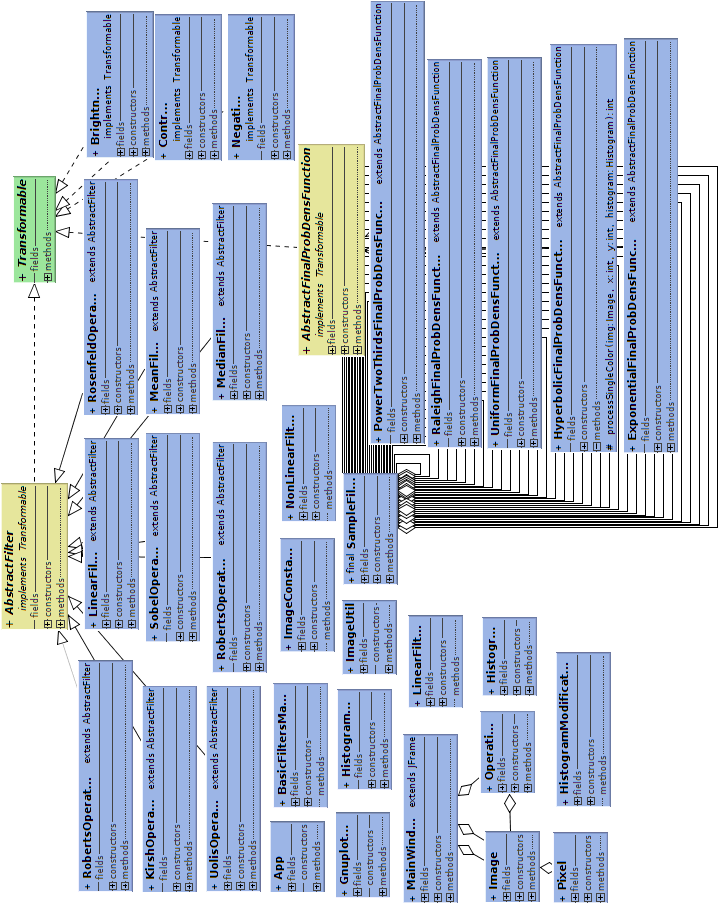
\includegraphics[scale=0.6]{img/uml_diagram.png}

\section{Materiały i metody}
Testowy zbiór przekształcanych obrazów można podzielić na 3 główne grupy:
\begin{itemize}
\item obrazy 1-bitowe
\begin{figure}%
    \centering
    \subfloat[Boat]{{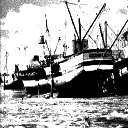
\includegraphics[width=2.5cm,height=2.5cm,keepaspectratio]{img/original/bit1/boatbw_small.png}}}%
    \qquad
    \subfloat[Girl]{{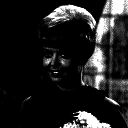
\includegraphics[width=2.5cm,height=2.5cm,keepaspectratio]{img/original/bit1/girlbw_small.png}}}%
    \qquad
    \subfloat[Lena]{{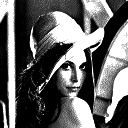
\includegraphics[width=2.5cm,height=2.5cm,keepaspectratio]{img/original/bit1/lenabw_small.png}}}%
    \qquad
    \subfloat[Mandril]{{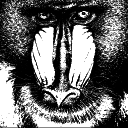
\includegraphics[width=2.5cm,height=2.5cm,keepaspectratio]{img/original/bit1/mandrilbw_small.png}}}%
    \caption{Testowe obrazy 1-bitowe}%
\end{figure}
\item obrazy 8-bitowe (w skali szarości)
\begin{figure}%
    \centering
    \subfloat[Aero]{{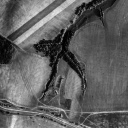
\includegraphics[width=2.5cm,height=2.5cm,keepaspectratio]{img/original/bit8/aero_small.png}}}%
    \qquad
    \subfloat[Bird]{{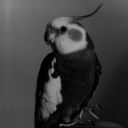
\includegraphics[width=2.5cm,height=2.5cm,keepaspectratio]{img/original/bit8/bird_small.png}}}%
    \qquad
    \subfloat[Boat]{{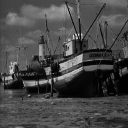
\includegraphics[width=2.5cm,height=2.5cm,keepaspectratio]{img/original/bit8/boat_small.png}}}%
    \qquad
    \subfloat[Bridge]{{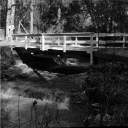
\includegraphics[width=2.5cm,height=2.5cm,keepaspectratio]{img/original/bit8/bridge_small.png}}}%
    \qquad
    \subfloat[Camera]{{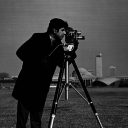
\includegraphics[width=2.5cm,height=2.5cm,keepaspectratio]{img/original/bit8/camera_small.png}}}%
    \qquad
    \subfloat[Lena]{{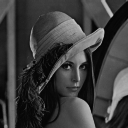
\includegraphics[width=2.5cm,height=2.5cm,keepaspectratio]{img/original/bit8/lena_small.png}}}%
    \qquad
    \subfloat[Mandril]{{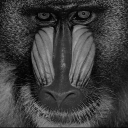
\includegraphics[width=2.5cm,height=2.5cm,keepaspectratio]{img/original/bit8/mandril_small.png}}}%
    \qquad
    \subfloat[Messer]{{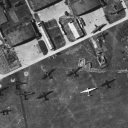
\includegraphics[width=2.5cm,height=2.5cm,keepaspectratio]{img/original/bit8/messer_small.png}}}%
    \qquad
    \subfloat[Pentagon]{{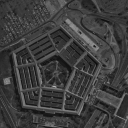
\includegraphics[width=2.5cm,height=2.5cm,keepaspectratio]{img/original/bit8/pentagon_small.png}}}%
    \caption{Testowe obrazy 8-bitowe}%
\end{figure}
\begin{figure}%
    \centering
    \subfloat[Impulsowy 1]{{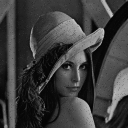
\includegraphics[width=2.5cm,height=2.5cm,keepaspectratio]{img/original/bit8/noise/lena_impulse1_small.png}}}%
    \qquad
    \subfloat[Impulsowy 2]{{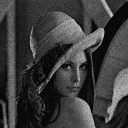
\includegraphics[width=2.5cm,height=2.5cm,keepaspectratio]{img/original/bit8/noise/lena_impulse2_small.png}}}%
    \qquad
    \subfloat[Impulsowy 3]{{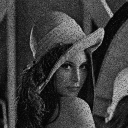
\includegraphics[width=2.5cm,height=2.5cm,keepaspectratio]{img/original/bit8/noise/lena_impulse3_small.png}}}%
    \qquad
    \subfloat[Normalny 1]{{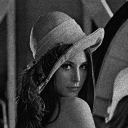
\includegraphics[width=2.5cm,height=2.5cm,keepaspectratio]{img/original/bit8/noise/lena_normal1_small.png}}}%
    \qquad
    \subfloat[Normalny 2]{{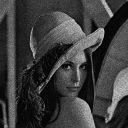
\includegraphics[width=2.5cm,height=2.5cm,keepaspectratio]{img/original/bit8/noise/lena_normal2_small.png}}}%
    \qquad
    \subfloat[Normalny 3]{{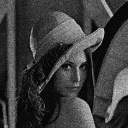
\includegraphics[width=2.5cm,height=2.5cm,keepaspectratio]{img/original/bit8/noise/lena_normal3_small.png}}}%
    \qquad
    \subfloat[Jednolity 1]{{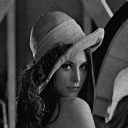
\includegraphics[width=2.5cm,height=2.5cm,keepaspectratio]{img/original/bit8/noise/lena_uniform1_small.png}}}%
    \qquad
    \subfloat[Jednolity 2]{{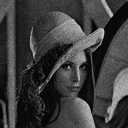
\includegraphics[width=2.5cm,height=2.5cm,keepaspectratio]{img/original/bit8/noise/lena_uniform2_small.png}}}%
    \qquad
    \subfloat[Jednolity 3]{{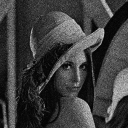
\includegraphics[width=2.5cm,height=2.5cm,keepaspectratio]{img/original/bit8/noise/lena_uniform3_small.png}}}%
    \caption{Testowe obrazy Lena 8-bitowe zaszumione}%
\end{figure}
\item obrazy 24-bitowe (RGB)
\begin{figure}%
    \centering
    \subfloat[Girl]{{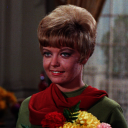
\includegraphics[width=2.5cm,height=2.5cm,keepaspectratio]{img/original/bit24/girlc_small.png}}}%
    \qquad
    \subfloat[Lena]{{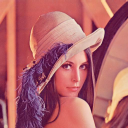
\includegraphics[width=2.5cm,height=2.5cm,keepaspectratio]{img/original/bit24/lenac_small.png}}}%
    \qquad
    \subfloat[Mandril]{{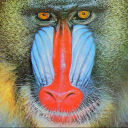
\includegraphics[width=2.5cm,height=2.5cm,keepaspectratio]{img/original/bit24/mandrilc_small.png}}}%
    \caption{Testowe obrazy 24-bitowe}%
\end{figure}
\begin{figure}%
    \centering
    \subfloat[Impulsowy 1]{{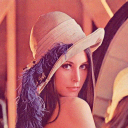
\includegraphics[width=2.5cm,height=2.5cm,keepaspectratio]{img/original/bit24/noise/lenac_impulse1_small.png}}}%
    \qquad
    \subfloat[Impulsowy 2]{{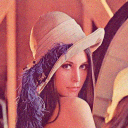
\includegraphics[width=2.5cm,height=2.5cm,keepaspectratio]{img/original/bit24/noise/lenac_impulse2_small.png}}}%
    \qquad
    \subfloat[Impulsowy 3]{{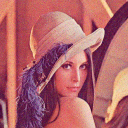
\includegraphics[width=2.5cm,height=2.5cm,keepaspectratio]{img/original/bit24/noise/lenac_impulse3_small.png}}}%
    \qquad
    \subfloat[Normalny 1]{{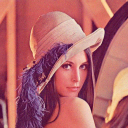
\includegraphics[width=2.5cm,height=2.5cm,keepaspectratio]{img/original/bit24/noise/lenac_normal1_small.png}}}%
    \qquad
    \subfloat[Normalny 2]{{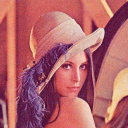
\includegraphics[width=2.5cm,height=2.5cm,keepaspectratio]{img/original/bit24/noise/lenac_normal2_small.png}}}%
    \qquad
    \subfloat[Normalny 3]{{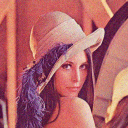
\includegraphics[width=2.5cm,height=2.5cm,keepaspectratio]{img/original/bit24/noise/lenac_normal3_small.png}}}%
    \qquad
    \subfloat[Jednolity 1]{{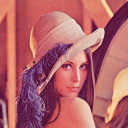
\includegraphics[width=2.5cm,height=2.5cm,keepaspectratio]{img/original/bit24/noise/lenac_uniform1_small.png}}}%
    \qquad
    \subfloat[Jednolity 2]{{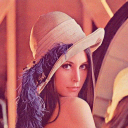
\includegraphics[width=2.5cm,height=2.5cm,keepaspectratio]{img/original/bit24/noise/lenac_uniform2_small.png}}}%
    \qquad
    \subfloat[Jednolity 3]{{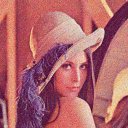
\includegraphics[width=2.5cm,height=2.5cm,keepaspectratio]{img/original/bit24/noise/lenac_uniform3_small.png}}}%
    \caption{Testowe obrazy Lena 24-bitowe zaszumione}%
\end{figure}
\end{itemize}

Badania zostały zrealizowane przy pomocy stworzonej aplikacji. Użytkownik definiował wejściowy obraz, który potem był poddawany wybranemu przez niego przekształceniu. Wyniki były zapisywane na dysku. Szczegółowa konfiguracja współczynników podczas transformacji zostanie podany w sekcji \textit{Wyniki}.

\section{Wyniki}
Poniżej przedstawione zostały efekty przeprowadzonych badań. Przeanalizowano wybrane obrazy 1-, 8- i 24-bitowe.

\subsection{Podstawowe operacje przetwarzania obrazu}
Sekcja przedstawia wyniki podstawowego przetwarzania obrazów - zmiany jasności, kontrastu oraz wyznaczenia negatywu.

\subsubsection{Zmiana jasności}
Poniżej przedstawione zostały wyniki zmiany jasności dla 3 wybranych obrazów.
\begin{figure}[H]%
    \centering
    \subfloat[k = -100]{{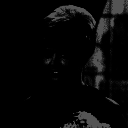
\includegraphics[width=2.5cm,height=2.5cm,keepaspectratio]{img/transformed/basic/brightness/brightness_girl_1_100_minus.png}}}%
    \qquad
    \subfloat[k = -50]{{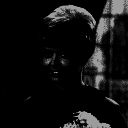
\includegraphics[width=2.5cm,height=2.5cm,keepaspectratio]{img/transformed/basic/brightness/brightness_girl_1_50_minus.png}}}%
      \qquad
    \subfloat[k = 50]{{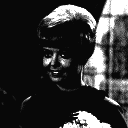
\includegraphics[width=2.5cm,height=2.5cm,keepaspectratio]{img/transformed/basic/brightness/brightness_girl_1_50_plus.png}}}%
    \qquad
    \subfloat[k = 100]{{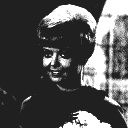
\includegraphics[width=2.5cm,height=2.5cm,keepaspectratio]{img/transformed/basic/brightness/brightness_girl_1_100_plus.png}}}%
    \caption{Zmiana jasności w obrazie Girl 1-bitowym}%
\end{figure}

\begin{figure}[H]%
    \centering
    \subfloat[k = -100]{{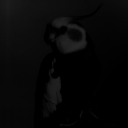
\includegraphics[width=2.5cm,height=2.5cm,keepaspectratio]{img/transformed/basic/brightness/brightness_bird_8_100_minus.png}}}%
    \qquad
    \subfloat[k = -50]{{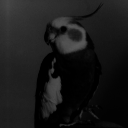
\includegraphics[width=2.5cm,height=2.5cm,keepaspectratio]{img/transformed/basic/brightness/brightness_bird_8_50_minus.png}}}%
      \qquad
    \subfloat[k = 50]{{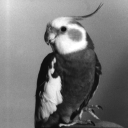
\includegraphics[width=2.5cm,height=2.5cm,keepaspectratio]{img/transformed/basic/brightness/brightness_bird_8_50_plus.png}}}%
    \qquad
    \subfloat[k = 100]{{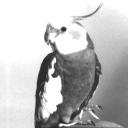
\includegraphics[width=2.5cm,height=2.5cm,keepaspectratio]{img/transformed/basic/brightness/brightness_bird_8_100_plus.png}}}%
    \caption{Zmiana jasności w obrazie Bird 8-bitowym}%
\end{figure}
\begin{figure}[H]%
    \centering
    \subfloat[k = -100]{{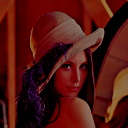
\includegraphics[width=2.5cm,height=2.5cm,keepaspectratio]{img/transformed/basic/brightness/brightness_lena_24_100_minus.png}}}%
    \qquad
    \subfloat[k = -50]{{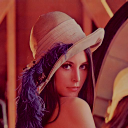
\includegraphics[width=2.5cm,height=2.5cm,keepaspectratio]{img/transformed/basic/brightness/brightness_lena_24_50_minus.png}}}%
      \qquad
    \subfloat[k = 50]{{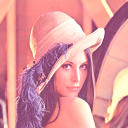
\includegraphics[width=2.5cm,height=2.5cm,keepaspectratio]{img/transformed/basic/brightness/brightness_lena_24_50_plus.png}}}%
    \qquad
    \subfloat[k = 100]{{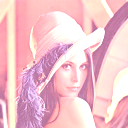
\includegraphics[width=2.5cm,height=2.5cm,keepaspectratio]{img/transformed/basic/brightness/brightness_lena_24_100_plus.png}}}%
    \caption{Zmiana jasności w obrazie Lena 24-bitowym}%
\end{figure}

\subsubsection{Zmiana kontrastu}
Poniżej przedstawione zostały wyniki zmiany kontrastu dla 3 wybranych obrazów.
\begin{figure}[H]%
    \centering
    \subfloat[k = 0.5]{{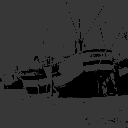
\includegraphics[width=2.5cm,height=2.5cm,keepaspectratio]{img/transformed/basic/contrast/contrast_boat_1_0_5.png}}}%
    \qquad
    \subfloat[k = 0.75]{{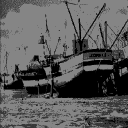
\includegraphics[width=2.5cm,height=2.5cm,keepaspectratio]{img/transformed/basic/contrast/contrast_boat_1_0_75.png}}}%
     \qquad
    \subfloat[k = 1.25]{{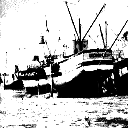
\includegraphics[width=2.5cm,height=2.5cm,keepaspectratio]{img/transformed/basic/contrast/contrast_boat_1_1_25.png}}}%
    \qquad
    \subfloat[k = 1.5]{{\includegraphics[width=2.5cm,height=2.5cm,keepaspectratio]{img/transformed/basic/contrast/contrast_boat_1_1_5.png}}}%
    \caption{Zmiana kontrastu w obrazie Boat 1-bitowym}%
\end{figure}

\begin{figure}[H]%
    \centering
    \subfloat[k = 0.5]{{\includegraphics[width=2.5cm,height=2.5cm,keepaspectratio]{img/transformed/basic/contrast/contrast_aero_8_0_5.png}}}%
    \qquad
    \subfloat[k = 0.75]{{\includegraphics[width=2.5cm,height=2.5cm,keepaspectratio]{img/transformed/basic/contrast/contrast_aero_8_0_75.png}}}%
     \qquad
    \subfloat[k = 1.25]{{\includegraphics[width=2.5cm,height=2.5cm,keepaspectratio]{img/transformed/basic/contrast/contrast_aero_8_1_25.png}}}%
    \qquad
    \subfloat[k = 1.5]{{\includegraphics[width=2.5cm,height=2.5cm,keepaspectratio]{img/transformed/basic/contrast/contrast_aero_8_1_5.png}}}%
    \caption{Zmiana kontrastu w obrazie Aero 8-bitowym}%
\end{figure}

\begin{figure}[H]%
    \centering
    \subfloat[k = 0.5]{{\includegraphics[width=2.5cm,height=2.5cm,keepaspectratio]{img/transformed/basic/contrast/contrast_mandril_24_0_5.png}}}%
    \qquad
    \subfloat[k = 0.75]{{\includegraphics[width=2.5cm,height=2.5cm,keepaspectratio]{img/transformed/basic/contrast/contrast_mandril_24_0_75.png}}}%
     \qquad
    \subfloat[k = 1.25]{{\includegraphics[width=2.5cm,height=2.5cm,keepaspectratio]{img/transformed/basic/contrast/contrast_mandril_24_1_25.png}}}%
    \qquad
    \subfloat[k = 1.5]{{\includegraphics[width=2.5cm,height=2.5cm,keepaspectratio]{img/transformed/basic/contrast/contrast_mandril_24_1_5.png}}}%
    \caption{Zmiana kontrastu w obrazie Mandril 24-bitowym}%
\end{figure}

\subsubsection{Wyznaczenie negatywu}
Poniżej przedstawione zostały wyniki wyznaczenia negatywu dla 3 wybranych obrazów.
\begin{figure}[H]%
    \centering
    \subfloat[Boat 1b]{{\includegraphics[width=2.5cm,height=2.5cm,keepaspectratio]{img/transformed/basic/negative/negative_boat_1.png}}}%
    \qquad
    \subfloat[Camera 8b]{{\includegraphics[width=2.5cm,height=2.5cm,keepaspectratio]{img/transformed/basic/negative/negative_camera_8.png}}}%
    \qquad
    \subfloat[Mandril 24b]{{\includegraphics[width=2.5cm,height=2.5cm,keepaspectratio]{img/transformed/basic/negative/negative_mandril_24.png}}}%
    \caption{Negatyw wybranych obrazów}%
\end{figure}


\subsection{Podstawowe filtry}
Sekcja przedstawia wyniki nałożenia na obrazy podstawowych filtrów - ze średnią arytmetyczną i medianowego.

\subsubsection{Filtr ze średnią arytmetyczną}
Poniżej przedstawione zostały wyniki nałożenia filtru ze średnią arytmetyczną na obraz Lena 8- i 24-bitowy dla szumów:
\begin{itemize}
\item Impulsowy 3
\item Jednolity 3
\item Normalny 3
\end{itemize}
W sprawozdaniu przedstawiono wyniki dla trzech masek: 3x3, 5x5 i 7x7.

\begin{figure}[H]%
    \centering
    \subfloat[Maska 3x3]{{\includegraphics[width=2.5cm,height=2.5cm,keepaspectratio]{img/transformed/basic_filters/mean/mean_filter_lena_8_impulse_3_3x3.png}}}%
    \qquad
    \subfloat[Maska 5x5]{{\includegraphics[width=2.5cm,height=2.5cm,keepaspectratio]{img/transformed/basic_filters/mean/mean_filter_lena_8_impulse_3_5x5.png}}}%
    \qquad
    \subfloat[Maska 7x7]{{\includegraphics[width=2.5cm,height=2.5cm,keepaspectratio]{img/transformed/basic_filters/mean/mean_filter_lena_8_impulse_3_7x7.png}}}%
    \caption{Wyniki nałożenia filtru ze średnią arytmetyczną na obraz Lena 8-bitowy, szum Impulsowy 3}%
\end{figure}

\begin{figure}[H]%
    \centering
    \subfloat[Maska 3x3]{{\includegraphics[width=2.5cm,height=2.5cm,keepaspectratio]{img/transformed/basic_filters/mean/mean_filter_lena_8_uniform_3_3x3.png}}}%
    \qquad
    \subfloat[Maska 5x5]{{\includegraphics[width=2.5cm,height=2.5cm,keepaspectratio]{img/transformed/basic_filters/mean/mean_filter_lena_8_uniform_3_5x5.png}}}%
    \qquad
    \subfloat[Maska 7x7]{{\includegraphics[width=2.5cm,height=2.5cm,keepaspectratio]{img/transformed/basic_filters/mean/mean_filter_lena_8_uniform_3_7x7.png}}}%
    \caption{Wyniki nałożenia filtru ze średnią arytmetyczną na obraz Lena 8-bitowy, szum Jednolity 3}%
\end{figure}

\begin{figure}[H]%
    \centering
    \subfloat[Maska 3x3]{{\includegraphics[width=2.5cm,height=2.5cm,keepaspectratio]{img/transformed/basic_filters/mean/mean_filter_lena_8_normal_3_3x3.png}}}%
    \qquad
    \subfloat[Maska 5x5]{{\includegraphics[width=2.5cm,height=2.5cm,keepaspectratio]{img/transformed/basic_filters/mean/mean_filter_lena_8_normal_3_5x5.png}}}%
    \qquad
    \subfloat[Maska7x7]{{\includegraphics[width=2.5cm,height=2.5cm,keepaspectratio]{img/transformed/basic_filters/mean/mean_filter_lena_8_normal_3_7x7.png}}}%
    \qquad
    \caption{Wyniki nałożenia filtru ze średnią arytmetyczną na obraz Lena 8-bitowy, szum Normalny 3}%
\end{figure}

\begin{figure}[H]%
    \centering
    \subfloat[Maska 3x3]{{\includegraphics[width=2.5cm,height=2.5cm,keepaspectratio]{img/transformed/basic_filters/mean/mean_filter_lena_24_impulse_3_3x3.png}}}%
    \qquad
    \subfloat[Maska 5x5]{{\includegraphics[width=2.5cm,height=2.5cm,keepaspectratio]{img/transformed/basic_filters/mean/mean_filter_lena_24_impulse_3_5x5.png}}}%
    \qquad
    \subfloat[Maska 7x7]{{\includegraphics[width=2.5cm,height=2.5cm,keepaspectratio]{img/transformed/basic_filters/mean/mean_filter_lena_24_impulse_3_7x7.png}}}%
    \caption{Wyniki nałożenia filtru ze średnią arytmetyczną na obraz Lena 24-bitowy, szum Impulsowy 3}%
\end{figure}

\begin{figure}[H]%
    \centering
    \subfloat[Maska 3x3]{{\includegraphics[width=2.5cm,height=2.5cm,keepaspectratio]{img/transformed/basic_filters/mean/mean_filter_lena_24_uniform_3_3x3.png}}}%
    \qquad
    \subfloat[Maska 5x5]{{\includegraphics[width=2.5cm,height=2.5cm,keepaspectratio]{img/transformed/basic_filters/mean/mean_filter_lena_24_uniform_3_5x5.png}}}%
    \qquad
    \subfloat[Maska 7x7]{{\includegraphics[width=2.5cm,height=2.5cm,keepaspectratio]{img/transformed/basic_filters/mean/mean_filter_lena_24_uniform_3_7x7.png}}}%
    \caption{Wyniki nałożenia filtru ze średnią arytmetyczną na obraz Lena 24-bitowy, szum Jednolity 3}%
\end{figure}

\begin{figure}[H]%
    \centering
    \subfloat[Maska 3x3]{{\includegraphics[width=2.5cm,height=2.5cm,keepaspectratio]{img/transformed/basic_filters/mean/mean_filter_lena_24_normal_3_3x3.png}}}%
    \qquad
    \subfloat[Maska 5x5]{{\includegraphics[width=2.5cm,height=2.5cm,keepaspectratio]{img/transformed/basic_filters/mean/mean_filter_lena_24_normal_3_5x5.png}}}%
    \qquad
    \subfloat[Maska7x7]{{\includegraphics[width=2.5cm,height=2.5cm,keepaspectratio]{img/transformed/basic_filters/mean/mean_filter_lena_24_normal_3_7x7.png}}}%
    \qquad
    \caption{Wyniki nałożenia filtru ze średnią arytmetyczną na obraz Lena 24-bitowy, szum Normalny 3}%
\end{figure}

\subsubsection{Filtr medianowy}
Poniżej przedstawione zostały wyniki nałożenia filtru medianowego na obraz Lena 8- i 24-bitowy dla szumów:
\begin{itemize}
\item Impulsowy 3
\item Jednolity 3
\item Normalny 3
\end{itemize}
W sprawozdaniu przedstawiono wyniki dla trzech masek: 3x3, 5x5 i 7x7.

\begin{figure}[H]%
    \centering
    \subfloat[Maska 3x3]{{\includegraphics[width=2.5cm,height=2.5cm,keepaspectratio]{img/transformed/basic_filters/median/median_filter_lena_8_impulse_3_3x3.png}}}%
    \qquad
    \subfloat[Maska 5x5]{{\includegraphics[width=2.5cm,height=2.5cm,keepaspectratio]{img/transformed/basic_filters/median/median_filter_lena_8_impulse_3_5x5.png}}}%
    \qquad
    \subfloat[Maska 7x7]{{\includegraphics[width=2.5cm,height=2.5cm,keepaspectratio]{img/transformed/basic_filters/median/median_filter_lena_8_impulse_3_7x7.png}}}%
    \caption{Wyniki nałożenia filtru medianowego na obraz Lena 8-bitowy, szum Impulsowy 3}%
\end{figure}

\begin{figure}[H]%
    \centering
    \subfloat[Maska 3x3]{{\includegraphics[width=2.5cm,height=2.5cm,keepaspectratio]{img/transformed/basic_filters/median/median_filter_lena_8_uniform_3_3x3.png}}}%
    \qquad
    \subfloat[Maska 5x5]{{\includegraphics[width=2.5cm,height=2.5cm,keepaspectratio]{img/transformed/basic_filters/median/median_filter_lena_8_uniform_3_5x5.png}}}%
    \qquad
    \subfloat[Maska 7x7]{{\includegraphics[width=2.5cm,height=2.5cm,keepaspectratio]{img/transformed/basic_filters/median/median_filter_lena_8_uniform_3_7x7.png}}}%
    \caption{Wyniki nałożenia filtru medianowego na obraz Lena 8-bitowy, szum Jednolity 3}%
\end{figure}

\begin{figure}[H]%
    \centering
    \subfloat[Maska 3x3]{{\includegraphics[width=2.5cm,height=2.5cm,keepaspectratio]{img/transformed/basic_filters/median/median_filter_lena_8_normal_3_3x3.png}}}%
    \qquad
    \subfloat[Maska 5x5]{{\includegraphics[width=2.5cm,height=2.5cm,keepaspectratio]{img/transformed/basic_filters/median/median_filter_lena_8_normal_3_5x5.png}}}%
    \qquad
    \subfloat[Maska 7x7]{{\includegraphics[width=2.5cm,height=2.5cm,keepaspectratio]{img/transformed/basic_filters/median/median_filter_lena_8_normal_3_7x7.png}}}%
    \qquad
    \caption{Wyniki nałożenia filtru medianowego na obraz Lena 8-bitowy, szum Normalny 3}%
\end{figure}

\begin{figure}[H]%
    \centering
    \subfloat[Maska 3x3]{{\includegraphics[width=2.5cm,height=2.5cm,keepaspectratio]{img/transformed/basic_filters/median/median_filter_lena_24_impulse_3_3x3.png}}}%
    \qquad
    \subfloat[Maska 5x5]{{\includegraphics[width=2.5cm,height=2.5cm,keepaspectratio]{img/transformed/basic_filters/median/median_filter_lena_24_impulse_3_5x5.png}}}%
    \qquad
    \subfloat[Maska 7x7]{{\includegraphics[width=2.5cm,height=2.5cm,keepaspectratio]{img/transformed/basic_filters/median/median_filter_lena_24_impulse_3_7x7.png}}}%
    \caption{Wyniki nałożenia filtru medianowego na obraz Lena 24-bitowy, szum Impulsowy 3}%
\end{figure}

\begin{figure}[H]%
    \centering
    \subfloat[Maska 3x3]{{\includegraphics[width=2.5cm,height=2.5cm,keepaspectratio]{img/transformed/basic_filters/median/median_filter_lena_24_uniform_3_3x3.png}}}%
    \qquad
    \subfloat[Maska 5x5]{{\includegraphics[width=2.5cm,height=2.5cm,keepaspectratio]{img/transformed/basic_filters/median/median_filter_lena_24_uniform_3_5x5.png}}}%
    \qquad
    \subfloat[Maska 7x7]{{\includegraphics[width=2.5cm,height=2.5cm,keepaspectratio]{img/transformed/basic_filters/median/median_filter_lena_24_uniform_3_7x7.png}}}%
    \caption{Wyniki nałożenia filtru medianowego na obraz Lena 24-bitowy, szum Jednolity 3}%
\end{figure}

\begin{figure}[H]%
    \centering
    \subfloat[Maska 3x3]{{\includegraphics[width=2.5cm,height=2.5cm,keepaspectratio]{img/transformed/basic_filters/median/median_filter_lena_24_normal_3_3x3.png}}}%
    \qquad
    \subfloat[Maska 5x5]{{\includegraphics[width=2.5cm,height=2.5cm,keepaspectratio]{img/transformed/basic_filters/median/median_filter_lena_24_normal_3_5x5.png}}}%
    \qquad
    \subfloat[Maska 7x7]{{\includegraphics[width=2.5cm,height=2.5cm,keepaspectratio]{img/transformed/basic_filters/median/median_filter_lena_24_normal_3_7x7.png}}}%
    \qquad
    \caption{Wyniki nałożenia filtru medianowego na obraz Lena 24-bitowy, szum Normalny 3}%
\end{figure}


\subsection{Modyfikacje obrazu w oparciu o histogram}
Sekcja przedstawia wyniki modyfikacji obrazów w oparciu o histogram. W celu porównania wyników, wszystkie operacje przeprowadzane były na obrazie 24-bitowym obrazie Lena. Poniżej przedstawiono histogramy kolorów obrazu oryginalnego.
\begin{figure}[H]%
    \centering
    \subfloat[CZERWONY]{{\includegraphics[width=6cm,height=6cm,keepaspectratio]{img/transformed/histogram/histogram_lena_24_red.png}}}%
    \qquad
    \subfloat[ZIELONY]{{\includegraphics[width=6cm,height=6cm,keepaspectratio]{img/transformed/histogram/histogram_lena_24_green.png}}}%
    \qquad
    \subfloat[NIEBIESKI]{{\includegraphics[width=6cm,height=6cm,keepaspectratio]{img/transformed/histogram/histogram_lena_24_blue.png}}}%
    \qquad
    \caption{Histogramy kolorów dla 24-bitowego obrazu Lena}%
\end{figure}

\subsubsection{Jednostajna wyjściowa gęstość prawdopodobieństwa}
Poniżej przedstawione zostały wyniki przetworzenia obrazu Lena 24-bitowego poprzez modyfikację histogramu jednostajną wyjściową gęstością prawdopodobieństwa.

\begin{figure}[H]%
    \centering
    \subfloat[gMin=10, gMax=240]{{\includegraphics[width=2.5cm,height=2.5cm,keepaspectratio]{img/transformed/histogram/uniform/histogram_uniform_lena_24_10_240.png}}}%
    \qquad
    \subfloat[gMin=50, gMax=200]{{\includegraphics[width=2.5cm,height=2.5cm,keepaspectratio]{img/transformed/histogram/uniform/histogram_uniform_lena_24_50_200.png}}}%
    \qquad
    \subfloat[gMin=90, gMax=160]{{\includegraphics[width=2.5cm,height=2.5cm,keepaspectratio]{img/transformed/histogram/uniform/histogram_uniform_lena_24_90_160.png}}}%
    \qquad
    \caption{Obraz Lena 24-bitowy przetworzony poprzez modyfikację histogramu jednostajną wyjściową gęstością prawdopodobieństwa}%
\end{figure}

\subsubsection{Wyjściowa gęstość prawdopodobieństwa podana wzorem Raleigha}
Poniżej przedstawione zostały wyniki przetworzenia obrazu Lena 24-bitowego poprzez modyfikację histogramu wyjściową gęstością prawdopodobieństwa podaną wzorem Raleigha.

\begin{figure}[H]%
    \centering
    \subfloat[gMin=10]{{\includegraphics[width=2.5cm,height=2.5cm,keepaspectratio]{img/transformed/histogram/raleigh/histogram_raleigh_lena_24_10.png}}}%
    \qquad
    \subfloat[gMin=50]{{\includegraphics[width=2.5cm,height=2.5cm,keepaspectratio]{img/transformed/histogram/raleigh/histogram_raleigh_lena_24_50.png}}}%
    \qquad
    \subfloat[gMin=90]{{\includegraphics[width=2.5cm,height=2.5cm,keepaspectratio]{img/transformed/histogram/raleigh/histogram_raleigh_lena_24_90.png}}}%
    \qquad
    \caption{Obraz Lena 24-bitowy przetworzony poprzez modyfikację histogramu wyjściową gęstością prawdopodobieństwa podaną wzorem Raleigha}%
\end{figure}

\subsubsection{Wyjściowa gęstość prawdopodobieństwa określona przez potęgę 2/3}
Poniżej przedstawione zostały wyniki przetworzenia obrazu Lena 24-bitowego poprzez modyfikację histogramu wyjściową gęstością prawdopodobieństwa określoną przez potęgę 2/3.

\begin{figure}[H]%
    \centering
    \subfloat[gMin=10, gMax=240]{{\includegraphics[width=2.5cm,height=2.5cm,keepaspectratio]{img/transformed/histogram/power_2_3/histogram_power_2_3_lena_24_10_240.png}}}%
    \qquad
    \subfloat[gMin=50, gMax=200]{{\includegraphics[width=2.5cm,height=2.5cm,keepaspectratio]{img/transformed/histogram/power_2_3/histogram_power_2_3_lena_24_50_200.png}}}%
    \qquad
    \subfloat[gMin=90, gMax=160]{{\includegraphics[width=2.5cm,height=2.5cm,keepaspectratio]{img/transformed/histogram/power_2_3/histogram_power_2_3_lena_24_90_160.png}}}%
    \qquad
    \caption{Obraz Lena 24-bitowy przetworzony poprzez modyfikację histogramu wyjściową gęstością prawdopodobieństwa określoną przez potęgę 2/3}%
\end{figure}

\subsubsection{Wyjściowa gęstość prawdopodobieństwa o postaci hiperbolicznej}
Poniżej przedstawione zostały wyniki przetworzenia obrazu Lena 24-bitowego poprzez modyfikację histogramu wyjściową gęstością prawdopodobieństwa o postaci hiperbolicznej.

\begin{figure}[H]%
    \centering
    \subfloat[gMin=10, gMax=240]{{\includegraphics[width=2.5cm,height=2.5cm,keepaspectratio]{img/transformed/histogram/hyperbolic/histogram_hyperbolic_lena_24_10_240.png}}}%
    \qquad
    \subfloat[gMin=50, gMax=200]{{\includegraphics[width=2.5cm,height=2.5cm,keepaspectratio]{img/transformed/histogram/hyperbolic/histogram_hyperbolic_lena_24_50_200.png}}}%
    \qquad
    \subfloat[gMin=90, gMax=160]{{\includegraphics[width=2.5cm,height=2.5cm,keepaspectratio]{img/transformed/histogram/hyperbolic/histogram_hyperbolic_lena_24_90_160.png}}}%
    \qquad
    \caption{Obraz Lena 24-bitowy przetworzony poprzez modyfikację histogramu wyjściową gęstością prawdopodobieństwa o postaci hiperbolicznej}%
\end{figure}

\subsection{Filtracja liniowa oparta o splot}
Sekcja przedstawia wyniki nałożenia na obrazy filtrów liniowych w oparciu o splot.

\subsubsection{Filtr dolnoprzepustowy}
Poniżej przedstawione zostały wyniki nałożenia filtru dolnoprzepustowego o różnych maskach na wybrane obrazy 8- i 24-bitowe. Wygląd masek znajduje się w sekcji \textit{Wprowadzenie}.

\begin{figure}[H]%
    \centering
    \subfloat[Maska 1]{{\includegraphics[width=2.5cm,height=2.5cm,keepaspectratio]{img/transformed/linear/low_pass/linear_low_pass_camera_8_1.png}}}%
    \qquad
    \subfloat[Maska 2]{{\includegraphics[width=2.5cm,height=2.5cm,keepaspectratio]{img/transformed/linear/low_pass/linear_low_pass_camera_8_2.png}}}%
    \qquad
    \subfloat[Maska 3]{{\includegraphics[width=2.5cm,height=2.5cm,keepaspectratio]{img/transformed/linear/low_pass/linear_low_pass_camera_8_3.png}}}%
    \caption{Wyniki nałożenia filtru dolnoprzepustowego o różnych maskach na obraz Camera 8-bitowy}%
\end{figure}

\begin{figure}[H]%
    \centering
    \subfloat[Maska 1]{{\includegraphics[width=2.5cm,height=2.5cm,keepaspectratio]{img/transformed/linear/low_pass/linear_low_pass_lena_24_1.png}}}%
    \qquad
    \subfloat[Maska 2]{{\includegraphics[width=2.5cm,height=2.5cm,keepaspectratio]{img/transformed/linear/low_pass/linear_low_pass_lena_24_1.png}}}%
    \qquad
    \subfloat[Maska 3]{{\includegraphics[width=2.5cm,height=2.5cm,keepaspectratio]{img/transformed/linear/low_pass/linear_low_pass_lena_24_1.png}}}%
    \caption{Wyniki nałożenia filtru dolnoprzepustowego o różnych maskach na obraz Lena 24-bitowy}%
\end{figure}

\subsubsection{Wyostrzanie krawędzi}
Poniżej przedstawione zostały wyniki wyostrzania krawędzi stosując różne maski na wybranych obrazach 8- i 24-bitowych. Wygląd masek znajduje się w sekcji \textit{Wprowadzenie}.

\begin{figure}[H]%
    \centering
    \subfloat[Maska 1]{{\includegraphics[width=2.5cm,height=2.5cm,keepaspectratio]{img/transformed/linear/edge_sharpening/linear_edge_sharpening_camera_8_1.png}}}%
    \qquad
    \subfloat[Maska 2]{{\includegraphics[width=2.5cm,height=2.5cm,keepaspectratio]{img/transformed/linear/edge_sharpening/linear_edge_sharpening_camera_8_2.png}}}%
    \qquad
    \subfloat[Maska 3]{{\includegraphics[width=2.5cm,height=2.5cm,keepaspectratio]{img/transformed/linear/edge_sharpening/linear_edge_sharpening_camera_8_3.png}}}%
    \caption{Wyniki wyostrzania krawędzi stosując różne maski na obrazie Camera 8-bitowym}%
\end{figure}

\begin{figure}[H]%
    \centering
    \subfloat[Maska 1]{{\includegraphics[width=2.5cm,height=2.5cm,keepaspectratio]{img/transformed/linear/edge_sharpening/linear_edge_sharpening_lena_24_1.png}}}%
    \qquad
    \subfloat[Maska 2]{{\includegraphics[width=2.5cm,height=2.5cm,keepaspectratio]{img/transformed/linear/edge_sharpening/linear_edge_sharpening_lena_24_1.png}}}%
    \qquad
    \subfloat[Maska 3]{{\includegraphics[width=2.5cm,height=2.5cm,keepaspectratio]{img/transformed/linear/edge_sharpening/linear_edge_sharpening_lena_24_1.png}}}%
    \caption{Wyniki wyostrzania krawędzi stosując różne maski na obrazie Lena 24-bitowym}%
\end{figure}

\subsubsection{Wydobywanie szczegółów z tła: N, NE, E, SE}
Poniżej przedstawione zostały wyniki wydobywania szczegółów z tła w kierunkach N, NE, E i SE na wybranych obrazach 8- i 24-bitowych. Wygląd masek znajduje się w sekcji \textit{Wprowadzenie}.

\begin{figure}[H]%
    \centering
    \subfloat[Kierunek N]{{\includegraphics[width=2.5cm,height=2.5cm,keepaspectratio]{img/transformed/linear/details_extraction_N_NE_S_SE/linear_details_extraction_camera_8_N.png}}}%
    \qquad
    \subfloat[Kierunek NE]{{\includegraphics[width=2.5cm,height=2.5cm,keepaspectratio]{img/transformed/linear/details_extraction_N_NE_S_SE/linear_details_extraction_camera_8_NE.png}}}%
    \qquad
    \subfloat[Kierunek E]{{\includegraphics[width=2.5cm,height=2.5cm,keepaspectratio]{img/transformed/linear/details_extraction_N_NE_S_SE/linear_details_extraction_camera_8_E.png}}}%
    \qquad
    \subfloat[Kierunek SE]{{\includegraphics[width=2.5cm,height=2.5cm,keepaspectratio]{img/transformed/linear/details_extraction_N_NE_S_SE/linear_details_extraction_camera_8_SE.png}}}%
    \caption{Wyniki wydobywania szczegółów z tła w kierunkach N, NE, E i SE na obrazie Camera 8-bitowym}%
\end{figure}

\begin{figure}[H]%
    \centering
    \subfloat[Kierunek N]{{\includegraphics[width=2.5cm,height=2.5cm,keepaspectratio]{img/transformed/linear/details_extraction_N_NE_S_SE/linear_details_extraction_lena_24_N.png}}}%
    \qquad
    \subfloat[Kierunek NE]{{\includegraphics[width=2.5cm,height=2.5cm,keepaspectratio]{img/transformed/linear/details_extraction_N_NE_S_SE/linear_details_extraction_lena_24_NE.png}}}%
    \qquad
    \subfloat[Kierunek E]{{\includegraphics[width=2.5cm,height=2.5cm,keepaspectratio]{img/transformed/linear/details_extraction_N_NE_S_SE/linear_details_extraction_lena_24_E.png}}}%
    \qquad
    \subfloat[Kierunek SE]{{\includegraphics[width=2.5cm,height=2.5cm,keepaspectratio]{img/transformed/linear/details_extraction_N_NE_S_SE/linear_details_extraction_lena_24_SE.png}}}%
    \caption{Wyniki wydobywania szczegółów z tła w kierunkach N, NE, E i SE na obrazie Lena 24-bitowym}%
\end{figure}

\subsubsection{Wydobywanie szczegółów z tła: S, SW, W, NW}
Poniżej przedstawione zostały wyniki wydobywania szczegółów z tła w kierunkach S, SW, W, NW na wybranych obrazach 8- i 24-bitowych. Wygląd masek znajduje się w sekcji \textit{Wprowadzenie}.

\begin{figure}[H]%
    \centering
    \subfloat[Kierunek S]{{\includegraphics[width=2.5cm,height=2.5cm,keepaspectratio]{img/transformed/linear/details_extraction_S_SW_W_NW/linear_details_extraction_camera_8_S.png}}}%
    \qquad
    \subfloat[Kierunek SW]{{\includegraphics[width=2.5cm,height=2.5cm,keepaspectratio]{img/transformed/linear/details_extraction_S_SW_W_NW/linear_details_extraction_camera_8_SW.png}}}%
    \qquad
    \subfloat[Kierunek W]{{\includegraphics[width=2.5cm,height=2.5cm,keepaspectratio]{img/transformed/linear/details_extraction_S_SW_W_NW/linear_details_extraction_camera_8_W.png}}}%
    \qquad
    \subfloat[Kierunek NW]{{\includegraphics[width=2.5cm,height=2.5cm,keepaspectratio]{img/transformed/linear/details_extraction_S_SW_W_NW/linear_details_extraction_camera_8_NW.png}}}%
    \caption{Wyniki wydobywania szczegółów z tła w kierunkach S, SW, W i NW na obrazie Camera 8-bitowym}%
\end{figure}

\begin{figure}[H]%
    \centering
    \subfloat[Kierunek S]{{\includegraphics[width=2.5cm,height=2.5cm,keepaspectratio]{img/transformed/linear/details_extraction_S_SW_W_NW/linear_details_extraction_lena_24_S.png}}}%
    \qquad
    \subfloat[Kierunek SW]{{\includegraphics[width=2.5cm,height=2.5cm,keepaspectratio]{img/transformed/linear/details_extraction_S_SW_W_NW/linear_details_extraction_lena_24_SW.png}}}%
    \qquad
    \subfloat[Kierunek W]{{\includegraphics[width=2.5cm,height=2.5cm,keepaspectratio]{img/transformed/linear/details_extraction_S_SW_W_NW/linear_details_extraction_lena_24_W.png}}}%
    \qquad
    \subfloat[Kierunek NW]{{\includegraphics[width=2.5cm,height=2.5cm,keepaspectratio]{img/transformed/linear/details_extraction_S_SW_W_NW/linear_details_extraction_lena_24_NW.png}}}%
    \caption{Wyniki wydobywania szczegółów z tła w kierunkach S, SW, W i NW na obrazie Lena 24-bitowym}%
\end{figure}

\subsubsection{Wydobywanie szczegółów z tła bez zdefiniowanego kierunku (laplasjan)}
Poniżej przedstawione zostały wyniki wydobywania szczegółów z tła bez zdefiniowanego kierunku na wybranych obrazach 8- i 24-bitowych. Wygląd masek znajduje się w sekcji \textit{Wprowadzenie}.

\begin{figure}[H]%
    \centering
    \subfloat[Maska 1]{{\includegraphics[width=2.5cm,height=2.5cm,keepaspectratio]{img/transformed/linear/details_extraction_no_direction_laplacian/linear_details_extraction_camera_8_laplacian_1.png}}}%
    \qquad
    \subfloat[Maska 2]{{\includegraphics[width=2.5cm,height=2.5cm,keepaspectratio]{img/transformed/linear/details_extraction_no_direction_laplacian/linear_details_extraction_camera_8_laplacian_1.png}}}%
    \qquad
    \subfloat[Maska 3]{{\includegraphics[width=2.5cm,height=2.5cm,keepaspectratio]{img/transformed/linear/details_extraction_no_direction_laplacian/linear_details_extraction_camera_8_laplacian_1.png}}}%
    \caption{Wyniki wydobywania szczegółów z tła bez zdefiniowanego kierunku na obrazie Camera 8-bitowym}%
\end{figure}

\begin{figure}[H]%
    \centering
    \subfloat[Maska 1]{{\includegraphics[width=2.5cm,height=2.5cm,keepaspectratio]{img/transformed/linear/details_extraction_no_direction_laplacian/linear_details_extraction_lena_24_laplacian_1.png}}}%
    \qquad
    \subfloat[Maska 2]{{\includegraphics[width=2.5cm,height=2.5cm,keepaspectratio]{img/transformed/linear/details_extraction_no_direction_laplacian/linear_details_extraction_lena_24_laplacian_1.png}}}%
    \qquad
    \subfloat[Maska 3]{{\includegraphics[width=2.5cm,height=2.5cm,keepaspectratio]{img/transformed/linear/details_extraction_no_direction_laplacian/linear_details_extraction_lena_24_laplacian_1.png}}}%
    \caption{Wyniki wwydobywania szczegółów z tła bez zdefiniowanego kierunku na obrazie Lena 24-bitowym}%
\end{figure}

\subsubsection{Identyfikowanie linii}
Poniżej przedstawione zostały wyniki identyfikacji linii z wybranych obrazów 8- i 24-bitowych. Wygląd masek znajduje się w sekcji \textit{Wprowadzenie}.

\begin{figure}[H]%
    \centering
    \subfloat[Poziomy]{{\includegraphics[width=2.5cm,height=2.5cm,keepaspectratio]{img/transformed/linear/line_identification/linear_line_identification_camera_8_horizontal.png}}}%
    \qquad
    \subfloat[Pionowy]{{\includegraphics[width=2.5cm,height=2.5cm,keepaspectratio]{img/transformed/linear/line_identification/linear_line_identification_camera_8_vertical.png}}}%
    \qquad
    \subfloat[Ukośny 1]{{\includegraphics[width=2.5cm,height=2.5cm,keepaspectratio]{img/transformed/linear/line_identification/linear_line_identification_camera_8_top_right_to_bottom_left.png}}}%
    \qquad
    \subfloat[Ukośny 2]{{\includegraphics[width=2.5cm,height=2.5cm,keepaspectratio]{img/transformed/linear/line_identification/linear_line_identification_camera_8_top_left_to_bottom_right.png}}}%
    \caption{Wyniki identyfikacji linii na obrazie Camera 8-bitowym}%
\end{figure}

\begin{figure}[H]%
    \centering
    \subfloat[Poziomy]{{\includegraphics[width=2.5cm,height=2.5cm,keepaspectratio]{img/transformed/linear/line_identification/linear_line_identification_lena_24_horizontal.png}}}%
    \qquad
    \subfloat[Pionowy]{{\includegraphics[width=2.5cm,height=2.5cm,keepaspectratio]{img/transformed/linear/line_identification/linear_line_identification_lena_24_vertical.png}}}%
    \qquad
    \subfloat[Ukośny 1]{{\includegraphics[width=2.5cm,height=2.5cm,keepaspectratio]{img/transformed/linear/line_identification/linear_line_identification_lena_24_top_right_to_bottom_left.png}}}%
    \qquad
    \subfloat[Ukośny 2]{{\includegraphics[width=2.5cm,height=2.5cm,keepaspectratio]{img/transformed/linear/line_identification/linear_line_identification_lena_24_top_left_to_bottom_right.png}}}%
    \caption{Wyniki identyfikacji linii na obrazie Lena 24-bitowym}%
\end{figure}

\subsection{Filtracja nieliniowa}
Sekcja przedstawia wyniki nałożenia na obrazy filtrów nieliniowych.

\subsubsection{Operator Robertsa (Wariant I)}
Poniżej przedstawione zostały wyniki zastosowania operatora Robertsa w I wariancie na wybranych obrazach 8- i 24-bitowych.

\begin{figure}[H]%
    \centering
    \subfloat[Bird 8b]{{\includegraphics[width=2.5cm,height=2.5cm,keepaspectratio]{img/transformed/nonlinear/roberts_1/non_linear_filter_roberts_v_I_bird_8.png}}}%
    \qquad
    \subfloat[Pentagon 8b]{{\includegraphics[width=2.5cm,height=2.5cm,keepaspectratio]{img/transformed/nonlinear/roberts_1/non_linear_filter_roberts_v_I_pentagon_8.png}}}%
    \qquad
    \subfloat[Girl 24b]{{\includegraphics[width=2.5cm,height=2.5cm,keepaspectratio]{img/transformed/nonlinear/roberts_1/non_linear_filter_roberts_v_I_girl_24.png}}}%
    \qquad
    \subfloat[Mandril 24b]{{\includegraphics[width=2.5cm,height=2.5cm,keepaspectratio]{img/transformed/nonlinear/roberts_1/non_linear_filter_roberts_v_I_mandril_24.png}}}%
    \qquad
    \caption{Wyniki zastosowania operatora Robertsa w I wariancie na wybranych obrazach 8- i 24-bitowych}%
\end{figure}

\subsubsection{Operator Robertsa (Wariant II)}
Poniżej przedstawione zostały wyniki zastosowania operatora Robertsa w II wariancie na wybranych obrazach 8- i 24-bitowych.

\begin{figure}[H]%
    \centering
    \subfloat[Bird 8b]{{\includegraphics[width=2.5cm,height=2.5cm,keepaspectratio]{img/transformed/nonlinear/roberts_2/non_linear_filter_roberts_v_II_bird_8.png}}}%
    \qquad
    \subfloat[Pentagon 8b]{{\includegraphics[width=2.5cm,height=2.5cm,keepaspectratio]{img/transformed/nonlinear/roberts_2/non_linear_filter_roberts_v_II_pentagon_8.png}}}%
    \qquad
    \subfloat[Girl 24b]{{\includegraphics[width=2.5cm,height=2.5cm,keepaspectratio]{img/transformed/nonlinear/roberts_2/non_linear_filter_roberts_v_II_girl_24.png}}}%
    \qquad
    \subfloat[Mandril 24b]{{\includegraphics[width=2.5cm,height=2.5cm,keepaspectratio]{img/transformed/nonlinear/roberts_2/non_linear_filter_roberts_v_II_mandril_24.png}}}%
    \qquad
    \caption{Wyniki zastosowania operatora Robertsa w I wariancie na wybranych obrazach 8- i 24-bitowych}%
\end{figure}

\subsubsection{Operator Sobela}
Poniżej przedstawione zostały wyniki zastosowania operatora Sobela na wybranych obrazach 8- i 24-bitowych.

\begin{figure}[H]%
    \centering
    \subfloat[Bird 8b]{{\includegraphics[width=2.5cm,height=2.5cm,keepaspectratio]{img/transformed/nonlinear/sobel/non_linear_filter_sobel_bird_8.png}}}%
    \qquad
    \subfloat[Pentagon 8b]{{\includegraphics[width=2.5cm,height=2.5cm,keepaspectratio]{img/transformed/nonlinear/sobel/non_linear_filter_sobel_pentagon_8.png}}}%
    \qquad
    \subfloat[Girl 24b]{{\includegraphics[width=2.5cm,height=2.5cm,keepaspectratio]{img/transformed/nonlinear/sobel/non_linear_filter_sobel_girl_24.png}}}%
    \qquad
    \subfloat[Mandril 24b]{{\includegraphics[width=2.5cm,height=2.5cm,keepaspectratio]{img/transformed/nonlinear/sobel/non_linear_filter_sobel_mandril_24.png}}}%
    \qquad
    \caption{Wyniki zastosowania operatora Sobela na wybranych obrazach 8- i 24-bitowych}%
\end{figure}

\subsubsection{Operator Kirsha}
Poniżej przedstawione zostały wyniki zastosowania operatora Kirsha na wybranych obrazach 8- i 24-bitowych.

\begin{figure}[H]%
    \centering
    \subfloat[Bird 8b]{{\includegraphics[width=2.5cm,height=2.5cm,keepaspectratio]{img/transformed/nonlinear/kirsh/non_linear_filter_kirsh_bird_8.png}}}%
    \qquad
    \subfloat[Pentagon 8b]{{\includegraphics[width=2.5cm,height=2.5cm,keepaspectratio]{img/transformed/nonlinear/kirsh/non_linear_filter_kirsh_pentagon_8.png}}}%
    \qquad
    \subfloat[Girl 24b]{{\includegraphics[width=2.5cm,height=2.5cm,keepaspectratio]{img/transformed/nonlinear/kirsh/non_linear_filter_kirsh_girl_24.png}}}%
    \qquad
    \subfloat[Mandril 24b]{{\includegraphics[width=2.5cm,height=2.5cm,keepaspectratio]{img/transformed/nonlinear/kirsh/non_linear_filter_kirsh_mandril_24.png}}}%
    \qquad
    \caption{Wyniki zastosowania operatora Kirsha na wybranych obrazach 8- i 24-bitowych}%
\end{figure}

\subsubsection{Operator Rosenfelda}
Poniżej przedstawione zostały wyniki zastosowania operatora Rosenfelda na wybranych obrazach 8- i 24-bitowych, w zależności od różnych parametrów R.

\begin{figure}[H]%
    \centering
    \subfloat[Bird 8b]{{\includegraphics[width=2.5cm,height=2.5cm,keepaspectratio]{img/transformed/nonlinear/rosenfeld/non_linear_filter_rosenfeld_bird_8_2.png}}}%
    \qquad
    \subfloat[Pentagon 8b]{{\includegraphics[width=2.5cm,height=2.5cm,keepaspectratio]{img/transformed/nonlinear/rosenfeld/non_linear_filter_rosenfeld_pentagon_8_2.png}}}%
    \qquad
    \subfloat[Girl 24b]{{\includegraphics[width=2.5cm,height=2.5cm,keepaspectratio]{img/transformed/nonlinear/rosenfeld/non_linear_filter_rosenfeld_girl_24_2.png}}}%
    \qquad
    \subfloat[Mandril 24b]{{\includegraphics[width=2.5cm,height=2.5cm,keepaspectratio]{img/transformed/nonlinear/rosenfeld/non_linear_filter_rosenfeld_mandril_24_2.png}}}%
    \qquad
    \caption{Wyniki zastosowania operatora Rosenfelfa na wybranych obrazach 8- i 24-bitowych, R = 2}%
\end{figure}

\begin{figure}[H]%
    \centering
    \subfloat[Bird 8b]{{\includegraphics[width=2.5cm,height=2.5cm,keepaspectratio]{img/transformed/nonlinear/rosenfeld/non_linear_filter_rosenfeld_bird_8_3.png}}}%
    \qquad
    \subfloat[Pentagon 8b]{{\includegraphics[width=2.5cm,height=2.5cm,keepaspectratio]{img/transformed/nonlinear/rosenfeld/non_linear_filter_rosenfeld_pentagon_8_3.png}}}%
    \qquad
    \subfloat[Girl 24b]{{\includegraphics[width=2.5cm,height=2.5cm,keepaspectratio]{img/transformed/nonlinear/rosenfeld/non_linear_filter_rosenfeld_girl_24_3.png}}}%
    \qquad
    \subfloat[Mandril 24b]{{\includegraphics[width=2.5cm,height=2.5cm,keepaspectratio]{img/transformed/nonlinear/rosenfeld/non_linear_filter_rosenfeld_mandril_24_3.png}}}%
    \qquad
    \caption{Wyniki zastosowania operatora Rosenfelfa na wybranych obrazach 8- i 24-bitowych, R = 3}%
\end{figure}

\begin{figure}[H]%
    \centering
    \subfloat[Bird 8b]{{\includegraphics[width=2.5cm,height=2.5cm,keepaspectratio]{img/transformed/nonlinear/rosenfeld/non_linear_filter_rosenfeld_bird_8_4.png}}}%
    \qquad
    \subfloat[Pentagon 8b]{{\includegraphics[width=2.5cm,height=2.5cm,keepaspectratio]{img/transformed/nonlinear/rosenfeld/non_linear_filter_rosenfeld_pentagon_8_4.png}}}%
    \qquad
    \subfloat[Girl 24b]{{\includegraphics[width=2.5cm,height=2.5cm,keepaspectratio]{img/transformed/nonlinear/rosenfeld/non_linear_filter_rosenfeld_girl_24_4.png}}}%
    \qquad
    \subfloat[Mandril 24b]{{\includegraphics[width=2.5cm,height=2.5cm,keepaspectratio]{img/transformed/nonlinear/rosenfeld/non_linear_filter_rosenfeld_mandril_24_4.png}}}%
    \qquad
    \caption{Wyniki zastosowania operatora Rosenfelfa na wybranych obrazach 8- i 24-bitowych, R = 4}%
\end{figure}

\subsubsection{Operator Uolisa}
Poniżej przedstawione zostały wyniki zastosowania operatora Uolisa na wybranych obrazach 8- i 24-bitowych.

\begin{figure}[H]%
    \centering
    \subfloat[Bird 8b]{{\includegraphics[width=2.5cm,height=2.5cm,keepaspectratio]{img/transformed/nonlinear/uolis/non_linear_filter_uolis_bird_8.png}}}%
    \qquad
    \subfloat[Pentagon 8b]{{\includegraphics[width=2.5cm,height=2.5cm,keepaspectratio]{img/transformed/nonlinear/uolis/non_linear_filter_uolis_pentagon_8.png}}}%
    \qquad
    \subfloat[Girl 24b]{{\includegraphics[width=2.5cm,height=2.5cm,keepaspectratio]{img/transformed/nonlinear/uolis/non_linear_filter_uolis_girl_24.png}}}%
    \qquad
    \subfloat[Mandril 24b]{{\includegraphics[width=2.5cm,height=2.5cm,keepaspectratio]{img/transformed/nonlinear/uolis/non_linear_filter_uolis_mandril_24.png}}}%
    \qquad
    \caption{Wyniki zastosowania operatora Uolisa na wybranych obrazach 8- i 24-bitowych}%
\end{figure}

\section{Dyskusja}
\noindent
Poniższa sekcja prezentuje interpretację uzyskanych wyników oraz wnioski. Opisano również napotkane problemy oraz możliwe sposoby ich rozwiązania.

\subsection{Podstawowe operacje przetwarzania obrazu}
\noindent
Przetworzenie obrazów podstawowymi operacjami przyniosło spodziewane rezultaty. 

\subsection{Podstawowe filtry}
Filtr ze średnią arytmetyczną umożliwia dokładne usunięcie szumu dopiero przy nałożeniu maski 5x5 (rys. 13-18b). Niestety, powoduje to również bardzo widoczne rozmycie obrazu.\\
\\
\indent
Filtr medianowy spełnia swoją role o wiele lepiej. Nadal widać różnicę pomiędzy obrazem oryginalnym, a odszumionym lecz porównując tę metodę z poprzednią (rys. 13-18 w porównaniu do rys. 19-24), widać wyraźną poprawę. Podobnie jak w przypadku filtru ze średnią arytmetyczną, po zastosowaniu większych masek, obraz staje się bardzo rozmazany.\\

\subsection{Modyfikacje obrazu w oparciu o histogram}
Modyfikacje obrazu w oparciu o histogram dały bardzo zbliżone rezultaty (rys. 26, 28, 29). Jedynym wyjątkiem jest przetworzenie poprzez modyfikację histogramu wyjściową gęstością prawdopodobieństwa podaną wzorem Raleigha. Wynikowe obrazy są negatywami (rys. 27).

\subsection{Filtracja liniowa oparta o splot}
Algorytm analizowanych filtrów polega na nałożeniu odpowiedniej maski na piksele oraz ich sąsiedztwo. Normalizacja wyników, w celu dokładniejszego wyświetlenia krawędzi, została zrealizowana poprzez dodanie współczynnika wynoszącego 0.7. Mnożone są przez niego wartości wszystkich pikseli wynikowych, jeżeli są mniejsze od maksymalnej.\\
\\
\indent
Filtr dolnoprzepustowy tłumi elementy o wysokiej częstotliwości i wygładza wejściowy obraz. Zarówno rysunek 8-bitowy (rys. 30), jak i 24-bitowy (rys. 31) dobrze prezentują to zachowanie.\\
\\
\indent
Wyostrzanie krawędzi dla obrazów w skali szarości przynosi najlepsze efekty przy zastosowaniu maski 2 (rys. 32b). Dla próbek w skali RGB (rys. 33), wyniki są porównywalne. \\
\\
\indent
Wydobywanie szczegółów z tła przynosi, zgodnie z oczekiwaniami, różne rezultaty przy analizie odmiennych obrazów. Wyraźnie można dostrzec korelację pomiędzy konturami elementów na obrazie a zastosowanym kierunkiem filtru (rys. 34-37).\\
\\
\indent
Wydobycie szczegółów z tła bez zdfiniowanego kierunku okazało się skomplikowanym zadaniem w przypadku testowych obrazów Camera i Lena. Algorytm zwrócił niesatysfakcjonujący wynik, odnajdując jedynie część konturów.\\
\\
\indent
Identyfikowanie linii, podobnie jak wydobywanie szczegółów z tła z zastosowanie konkretnego kierunku poszukiwań, jest ściśle związane z analziowanym obrazem. Widać to między innymi na identyfikacji pionowej obrazu Camera (rys. 40b) oraz ukośnej 1 próbki Lena (rys. 41c).\\ 
\\
\indent 
W celu zoptymalizowania filtrów z powyższej sekcji pod względem czasowym i pamięciowym, można zastosować następujące rozwiązania:
\begin{itemize}
\item w przypadku masek posiadających zera, można zarezerwować mniejszą ilość pamięci na jej przechowywanie, pomijając te elementy; podczas działania program, nie powinien on wykonywać podwójnego fora na pikselu (aby obliczyć wartości z całej maski nxn), lecz wybierać tych sąsiadów, którzy faktycznie mają wpływ na finalny wynik
\item podobnie jak w poprzednim punkcie można postąpić z elementami maski o wartościach 1 lub -1; zamiast wymnażać je przez wartość piksela i dopiero po tej operacji dodawać go do sumy, można pominąć zbędny krok  
\end{itemize}

\subsection{Filtracja nieliniowa}
Filtracja nieliniowa umożliwia znalezienie krawędzi elementów, bez względu na ich położenie względem osi XOY.\\
\\
\indent
Operator Robertsa, a zwłaszcza jego drugi wariant, bardzo dokładnie pokazuje wszystkie wyraźne, lokalne zmiany w natężeniu barw. Widać to szczególnie dobrze na rysunkach przedstawiających ptaka (rys. 43a) oraz dziewczynę (rys. 43c).\\
\\
\indent
Operator Sobela również dobrze sobie radzi z odnajdywaniem krawędzi, jednakże oznacza je o wiele grubszymi liniami. Ponieważ bierze pod uwagę większe sąsiedztwo pikseli niż operator Robertsa, dokładnie odwzorowuje kontury elementów pod warunkiem, że nie są one położone blisko siebie (rys. 44a i rys.44b). W momencie w którym obraz na wejściu nie ma wyraźnych krawędzi znacznie oddalonych od siebie (rys. 44d), wynik jest niesatysfakcjonujący.\\
\\
\indent
Zastosowanie operatora Kirsha przynosi efekty podobne do operatora Sobela, jednakże jezcze trudniej można się doszukać oryginalnych konturów. Dobrze obrazuje to przykład Pentagonu (rys. 45b) oraz mandryla (rys. 45d). Ze względu na dużą jasność wszystkich wyników, dane wyjściowe możnaby poddać normalizacji.\\
\\
\indent
Operator Rosenfelda odnajduje krawędzi (rys. 46b) lecz tworzy niepotrzebny szum tła (rys. 46a). Zwiększanie parametru R powoduje pogrubianie wynikowych linii. 
\\
\indent
Wynik przekształcenia operatorem Uolisa został znormalizowany poprzez pomnożenie wartości każdego piksela przez liczbę 10. Bez tej operacji rezultat był nieczytelny. Po transformacji, wynik prezentuje najbardziej wyraziste krawędzie (rys. 49).

\section{Wnioski}
Podsumowując, do usuwania szumów nie powinno się stosować filtru ze średnią arytmetyczną, ponieważ filr medianiowy daje lepsze rezultaty. Trzeba jednak pamiętać, aby nie nałożyć zbyt dużej maski, ponieważ otrzymany obraz może się okazać zbyt rozmazany.\\
\\
\indent
Przetworzenie obrazu poprzez modyfikację histogramu jednostajną wyjściową gęstością prawdopodobieństwa, wyjściowa gęstością prawdopodobieństwa określoną przez potęgę 2/3 oraz wyjściową gęstością prawdopodobieństwa o postaci hiperbolicznej daje bardzo zbliżone rezultaty.\\
\\
\indent
Filtracja liniowa oparta o splot potrafi dać bardzo dobre rezultaty wyszukiwania krawędzi pod warunkiem, że szukamy ich w konretnych kierunkach.\\
\\
\indent
Filtracja nieliniowa daje o wiele lepsze efekty. Szczególnie operator Robertsa w wariancie 2 oraz operator Sobela pozwalają na bardzo dokładne wyróżnienie wszystkich krawędzi.

\begin{thebibliography}{1}
\bibitem{instruction_pol}\text{$http://ftims.edu.p.lodz.pl/pluginfile.php/18220/mod\_resource/content/1/$}\\
\text{$Zadanie1.pdf, 2015$}
\bibitem{instruction_ang}\text{$http://ics.p.lodz.pl/~tomczyk/available/po\_en/second.html, 2015$}
\bibitem{instruction_latex}\text{$https://en.wikibooks.org/wiki/LaTeX/Mathematics, 2015$}
\bibitem{doc_linear_fitering}\text{$https://pl.wikipedia.org/wiki/Filtracja\_obraz\%C3\%B3w, 2015$}
\end{thebibliography}
\end{document}
